
\subsection{Expérience 3}
Après voir l'aspect de $ t_{max} $ et du nombre des fourmis $ m $ aspects du \textbf{AS algorithme}, j'ai fixé le nombre des fourmis sur 40 et j'ai fait les statistiques pour faire la comparaison sur le STD et le Mean exécution of the execution times and the journey path of the AS and Greedy algorithm.
et Comme vous avez demandé dans le point (4) , la séquence est bien présenté dans les figure ci-dessous.
\subsection*{ \centering Exp. 2 on cities.dat \comm{figure of Pathofcities cities of exp 2}}

\begin{figure}[H]
	\begin{minipage}[t]{0.45\linewidth}
	\centering
	\includegraphics[width=\textwidth]{\Pathofcities/path.eps}
	\caption{Path journey}\label{fig:Pathofcities:path}
	
	\end{minipage}\hfill
	\begin{minipage}[t]{0.45\linewidth}
	\centering
	\includegraphics[width=\textwidth]{\Pathofcities/AS_1_5AS_ExecTimeAndMeanSTDWith_execVariation.eps}
	\caption{Variation of the execution time VS the \# of ants (20$\stackrel{step=20}{\rightarrow}$100) in each execution (1$\stackrel{step=1}{\rightarrow}$ 5)}
	\label{fig:Pathofcities:AS_1_5AS_ExecTimeAndMeanSTDWith_execVariation}
	\end{minipage}
	\flushleft
	\begin{minipage}[t]{0.45\linewidth}
	\centering
	\includegraphics[width=1.5\textwidth,height=.9\textwidth]{\Pathofcities/AS_BestCost_Varying_Iteration_and_nbAnts.eps}
	\caption{Best cost VS Ants number variation with $\alpha$=1, $ \beta $ = 5}
	\label{fig:Pathofcities:AS_BestCost_Varying_Iteration_and_nbAnts}
	\end{minipage}
%%	\vspace{length}
\end{figure}\flushright
	\begin{minipage}[t]{0.9\linewidth}
	\vspace{-9mm}
	\begin{table}[H]
	\label{tab:Pathofcities:expdeux}
	\begin{tabular}{lllll}
	\cline{1-2}
	\multicolumn{1}{|l|}{Best Costs results for experience 2 on cities.dat }                                                           &  \multicolumn{1}{l|}{Elapsed Time, Mean, STD}                                             &  &  &  \\ \cline{1-2}
	\multicolumn{1}{|l|}{\begin{tiny}\begin{tabular}{|l|c|c|c|c|c|c|c|c|c|c|}
\hline
&\textbf{It :1}&\textbf{It :2}&\textbf{It :3}&\textbf{It :4}&\textbf{It :5}&\textbf{It :6}&\textbf{It :7}&\textbf{It :8}&\textbf{It :9}&\textbf{It :10}\\\hline
\textbf{exec :1}&28.07&28.07&28.07&28.07&28.07&28.07&28.07&27.52&27.52&27.52\\\hline
\textbf{exec :2}&28.86&28.86&28.86&28.86&28.86&28.86&27.52&27.52&27.52&27.52\\\hline
\textbf{exec :3}&29.16&29.13&28.05&28.05&28.05&28.05&28.05&28.05&27.72&27.52\\\hline
\textbf{exec :4}&29.05&27.52&27.52&27.52&27.52&27.52&27.52&27.52&27.52&27.52\\\hline
\textbf{exec :5}&29.47&27.52&27.52&27.52&27.52&27.52&27.52&27.52&27.52&27.52\\\hline
\textbf{exec :6}&28.66&28.09&27.52&27.52&27.52&27.52&27.52&27.52&27.52&27.52\\\hline
\textbf{exec :7}&28.05&27.72&27.52&27.52&27.52&27.52&27.52&27.52&27.52&27.52\\\hline
\textbf{exec :8}&27.72&27.52&27.52&27.52&27.52&27.52&27.52&27.52&27.52&27.52\\\hline
\textbf{exec :9}&27.52&27.52&27.52&27.52&27.52&27.52&27.52&27.52&27.52&27.52\\\hline
\textbf{exec :10}&27.52&27.52&27.52&27.52&27.52&27.52&27.52&27.52&27.52&27.52\\\hline
\end{tabular}
\end{tiny}} & \multicolumn{1}{l|}{\begin{tiny}\begin{tabular}{|l|c|}
\hline
&\textbf{Elapsed time}\\\hline
\textbf{exec :1}&0.29\\\hline
\textbf{exec :2}&0.54\\\hline
\textbf{exec :3}&0.78\\\hline
\textbf{exec :4}&1.02\\\hline
\textbf{exec :5}&1.27\\\hline
\textbf{exec :6}&2.48\\\hline
\textbf{exec :7}&3.73\\\hline
\textbf{exec :8}&4.96\\\hline
\textbf{exec :9}&6.16\\\hline
\textbf{exec :10}&12.40\\\hline
\textbf{ Mean}&3.36\\\hline
\textbf{ STD}&3.75\\\hline
\end{tabular}
\end{tiny} } &  &  &  \\ \cline{1-2}
	&     &  &  &  \\
	&     &  &  & 
	\end{tabular}
	\caption{Results of experience 2 on cities.dat}
	\end{table}
	\end{minipage}

%%\end{figure}

\subsection*{ \centering Exp. 2 on cities2.dat \comm{figure of Pathofcitiesdeux cities2 of exp 2}}
\begin{figure}[H]
	\begin{minipage}[t]{0.45\linewidth}
	\centering
	\includegraphics[width=\textwidth]{\Pathofcitiesdeux/path.eps}
	\caption{Path journey}\label{fig:Pathofcitiesdeux:path}
	
	\end{minipage}\hfill
	\begin{minipage}[t]{0.45\linewidth}
	\centering
	\includegraphics[width=\textwidth]{\Pathofcitiesdeux/AS_1_5AS_ExecTimeAndMeanSTDWith_execVariation.eps}
	\caption{Variation of the execution time VS the \# of ants (20$\stackrel{step=20}{\rightarrow}$100) in each execution (1$\stackrel{step=1}{\rightarrow}$ 5)}
	\label{fig:Pathofcitiesdeux:AS_1_5AS_ExecTimeAndMeanSTDWith_execVariation}
	\end{minipage}
	\flushleft
	\begin{minipage}[t]{0.45\linewidth}
	\centering
	\includegraphics[width=1.5\textwidth,height=.9\textwidth]{\Pathofcitiesdeux/AS_BestCost_Varying_Iteration_and_nbAnts.eps}
	\caption{Best cost VS Ants number variation with $\alpha$=1, $ \beta $ = 5}
	\label{fig:Pathofcitiesdeux:AS_BestCost_Varying_Iteration_and_nbAnts}
	\end{minipage}
%%	\vspace{length}
\end{figure}\flushright
	\begin{minipage}[t]{0.9\linewidth}
	\vspace{-9mm}
	\begin{table}[H]
	\label{tab:Pathofcitiesdeux:expdeux}
	\begin{tabular}{lllll}
	\cline{1-2}
	\multicolumn{1}{|l|}{Best Costs results for experience 2 on cities.dat }                                                           &  \multicolumn{1}{l|}{Elapsed Time, Mean, STD}                                             &  &  &  \\ \cline{1-2}
	\multicolumn{1}{|l|}{\begin{tiny}\begin{tabular}{|l|c|c|c|c|c|c|c|c|c|c|}
\hline
&\textbf{It :1}&\textbf{It :2}&\textbf{It :3}&\textbf{It :4}&\textbf{It :5}&\textbf{It :6}&\textbf{It :7}&\textbf{It :8}&\textbf{It :9}&\textbf{It :10}\\\hline
\textbf{exec :1}&3.37&3.26&3.08&3.08&3.05&3.05&3.05&3.05&3.05&3.05\\\hline
\textbf{exec :2}&3.35&3.15&2.91&2.91&2.91&2.91&2.91&2.91&2.91&2.91\\\hline
\textbf{exec :3}&3.21&3.21&3.11&3.11&3.10&2.99&2.99&2.99&2.99&2.99\\\hline
\textbf{exec :4}&3.25&3.13&3.11&2.93&2.93&2.93&2.93&2.93&2.93&2.93\\\hline
\textbf{exec :5}&3.20&2.95&2.95&2.95&2.95&2.95&2.95&2.95&2.95&2.95\\\hline
\textbf{exec :6}&3.23&3.10&3.10&3.10&3.10&3.10&3.10&3.10&3.02&3.02\\\hline
\textbf{exec :7}&3.21&3.21&3.10&3.00&3.00&3.00&3.00&3.00&2.96&2.96\\\hline
\textbf{exec :8}&3.21&3.06&3.06&3.05&3.03&2.98&2.98&2.98&2.98&2.98\\\hline
\textbf{exec :9}&3.44&3.05&3.03&2.97&2.97&2.97&2.97&2.97&2.97&2.97\\\hline
\textbf{exec :10}&3.31&3.02&3.02&3.02&3.02&3.01&3.01&3.01&3.01&3.01\\\hline
\end{tabular}
\end{tiny}} & \multicolumn{1}{l|}{\begin{tiny}\begin{tabular}{|l|c|}
\hline
&\textbf{Elapsed time}\\\hline
\textbf{exec :1}&0.94\\\hline
\textbf{exec :2}&1.68\\\hline
\textbf{exec :3}&2.42\\\hline
\textbf{exec :4}&3.17\\\hline
\textbf{exec :5}&3.90\\\hline
\textbf{exec :6}&7.60\\\hline
\textbf{exec :7}&11.29\\\hline
\textbf{exec :8}&14.93\\\hline
\textbf{exec :9}&18.65\\\hline
\textbf{exec :10}&36.72\\\hline
\textbf{ Mean}&10.13\\\hline
\textbf{ STD}&11.12\\\hline
\end{tabular}
\end{tiny} } &  &  &  \\ \cline{1-2}
	&     &  &  &  \\
	&     &  &  & 
	\end{tabular}
	\caption{Results of experience 2 on cities2.dat}
	\end{table}
	\end{minipage}

\subsection*{ \centering Exp. 2 on rand 50.dat\comm{figure of Pathofcinq of exp 2}}
\begin{figure}[H]
		\begin{minipage}[t]{0.45\linewidth}
		\centering
		\includegraphics[width=\textwidth]{\Pathofcinq/path.eps}
		\caption{Path journey}\label{fig:Pathofcinq:path}
		
		\end{minipage}\hfill
		\begin{minipage}[t]{0.45\linewidth}
		\centering
		\includegraphics[width=\textwidth]{\Pathofcinq/AS_1_5AS_ExecTimeAndMeanSTDWith_execVariation.eps}
		\caption{Variation of the execution time VS the \# of ants (20$\stackrel{step=20}{\rightarrow}$100) in each execution (1$\stackrel{step=1}{\rightarrow}$ 5)}
		\label{fig:Pathofcinq:AS_1_5AS_ExecTimeAndMeanSTDWith_execVariation}
		\end{minipage}
	\flushleft
		\begin{minipage}[t]{0.45\linewidth}
		\centering
		\includegraphics[width=1.5\textwidth]{\Pathofcinq/AS_BestCost_Varying_Iteration_and_nbAnts.eps}
		\caption{Best cost VS Ants number variation with $\alpha$=1, $ \beta $ = 5}
		\label{fig:Pathofcinq:AS_BestCost_Varying_Iteration_and_nbAnts}
		\end{minipage}
\end{figure}
		\begin{minipage}[t]{0.9\linewidth}
		\vspace{-9mm}
		\begin{table}[H]
		\label{tab:Pathofcinq:expdeux}
		\begin{tabular}{lllll}
		\cline{1-2}
		\multicolumn{1}{|l|}{Best Costs results for experience 2}                                                           &  \multicolumn{1}{l|}{Elapsed Time, Mean, STD}                                             &  &  &  \\ \cline{1-2}
		\multicolumn{1}{|l|}{\begin{tiny}\begin{tabular}{|l|c|c|c|c|c|c|c|c|c|c|}
\hline
&\textbf{It :1}&\textbf{It :2}&\textbf{It :3}&\textbf{It :4}&\textbf{It :5}&\textbf{It :6}&\textbf{It :7}&\textbf{It :8}&\textbf{It :9}&\textbf{It :10}\\\hline
\textbf{exec :1}&678.98&678.98&678.98&673.98&673.98&673.98&673.98&673.98&670.30&670.30\\\hline
\textbf{exec :2}&700.62&687.16&686.29&686.29&686.29&656.58&656.58&656.58&656.58&656.58\\\hline
\textbf{exec :3}&680.99&644.35&644.35&644.35&644.35&644.35&644.35&644.35&644.35&644.35\\\hline
\textbf{exec :4}&677.23&665.56&665.56&665.56&665.56&665.56&632.39&632.39&632.39&632.39\\\hline
\textbf{exec :5}&683.50&683.30&650.17&650.17&650.17&614.01&614.01&614.01&614.01&614.01\\\hline
\textbf{exec :6}&643.11&643.11&635.79&635.79&635.79&635.79&635.79&635.79&635.79&635.79\\\hline
\textbf{exec :7}&632.45&632.45&632.45&630.20&630.20&609.73&609.73&609.73&609.73&609.73\\\hline
\textbf{exec :8}&634.94&634.94&618.14&618.14&618.14&618.14&618.14&618.14&618.14&618.14\\\hline
\textbf{exec :9}&646.33&645.36&627.11&617.99&617.99&617.99&617.99&617.99&617.99&617.99\\\hline
\textbf{exec :10}&647.03&638.44&638.44&630.35&615.00&615.00&615.00&615.00&615.00&615.00\\\hline
\end{tabular}
\end{tiny}} & \multicolumn{1}{l|}{\begin{tiny}\begin{tabular}{|l|c|}
\hline
&\textbf{Elapsed time}\\\hline
\textbf{exec :1}&0.96\\\hline
\textbf{exec :2}&1.70\\\hline
\textbf{exec :3}&2.46\\\hline
\textbf{exec :4}&3.21\\\hline
\textbf{exec :5}&3.96\\\hline
\textbf{exec :6}&7.69\\\hline
\textbf{exec :7}&11.38\\\hline
\textbf{exec :8}&15.04\\\hline
\textbf{exec :9}&19.05\\\hline
\textbf{exec :10}&38.17\\\hline
\textbf{ Mean}&10.36\\\hline
\textbf{ STD}&11.53\\\hline
\end{tabular}
\end{tiny} } &  &  &  \\ \cline{1-2}
																						  &                                                                     &  &  &  \\
																						  &                                                                     &  &  & 
		\end{tabular}
		\caption{Results of experience 2 on rand50.dat}
		\end{table}
		\end{minipage}

\subsection*{ \centering Exp. 2 on rand 60.dat\comm{figure of Pathofsix of exp 2}}
\comm{}
\begin{figure}[H]
		\begin{minipage}[t]{0.45\linewidth}
		\centering
		\includegraphics[width=\textwidth]{\Pathofsix/path.eps}
		\caption{Path journey}\label{fig:Pathofsix:path}
		
		\end{minipage}\hfill
		\begin{minipage}[t]{0.45\linewidth}
		\centering
		\includegraphics[width=\textwidth]{\Pathofsix/AS_1_5AS_ExecTimeAndMeanSTDWith_execVariation.eps}
		\caption{Variation of the execution time VS the \# of ants (20$\stackrel{step=20}{\rightarrow}$100) in each execution (1$\stackrel{step=1}{\rightarrow}$ 5)}
		\label{fig:Pathofsix:AS_1_5AS_ExecTimeAndMeanSTDWith_execVariation}
		\end{minipage}
		\flushleft
		\begin{minipage}[t]{0.45\linewidth}
		\centering
		\includegraphics[width=1.5\textwidth]{\Pathofsix/AS_BestCost_Varying_Iteration_and_nbAnts.eps}
		\caption{Best cost VS Ants number variation with $\alpha$=1, $ \beta $ = 5}
		\label{fig:Pathofsix:AS_BestCost_Varying_Iteration_and_nbAnts}
		\end{minipage}
\end{figure}
		\begin{minipage}[t]{0.9\linewidth}
		\vspace{-9mm}
		\begin{table}[H]
		\label{tab:Pathofsix:expdeux}
		\begin{tabular}{lllll}
		\cline{1-2}
		\multicolumn{1}{|l|}{Best Costs results for experience 2}                                                           &  \multicolumn{1}{l|}{Elapsed Time, Mean, STD}                                             &  &  &  \\ \cline{1-2}
		\multicolumn{1}{|l|}{\begin{tiny}\begin{tabular}{|l|c|c|c|c|c|c|c|c|c|c|}
\hline
&\textbf{It :1}&\textbf{It :2}&\textbf{It :3}&\textbf{It :4}&\textbf{It :5}&\textbf{It :6}&\textbf{It :7}&\textbf{It :8}&\textbf{It :9}&\textbf{It :10}\\\hline
\textbf{exec :1}&722.04&722.04&722.04&717.16&717.16&682.93&682.93&682.93&682.93&682.93\\\hline
\textbf{exec :2}&714.47&714.47&705.30&705.30&705.30&705.30&703.25&703.25&699.32&681.75\\\hline
\textbf{exec :3}&745.85&701.98&701.98&701.98&701.98&701.98&701.98&699.66&699.66&699.66\\\hline
\textbf{exec :4}&714.25&667.50&667.50&657.11&657.11&657.11&657.11&657.11&657.11&657.11\\\hline
\textbf{exec :5}&677.45&677.45&677.45&677.45&677.45&677.45&677.45&677.45&677.45&677.45\\\hline
\textbf{exec :6}&668.72&668.72&668.72&668.72&668.72&668.72&668.72&668.72&668.72&668.72\\\hline
\textbf{exec :7}&687.25&645.63&645.63&645.63&645.63&645.63&645.63&645.63&645.63&645.63\\\hline
\textbf{exec :8}&689.81&664.05&664.05&664.05&655.03&655.03&655.03&655.03&655.03&655.03\\\hline
\textbf{exec :9}&677.43&677.43&677.43&664.47&664.47&649.08&649.08&649.08&649.08&649.08\\\hline
\textbf{exec :10}&694.51&668.56&656.68&656.68&656.68&650.95&650.95&650.95&650.95&650.95\\\hline
\end{tabular}
\end{tiny}} & \multicolumn{1}{l|}{\begin{tiny}\begin{tabular}{|l|c|}
\hline
&\textbf{Elapsed time}\\\hline
\textbf{exec :1}&2.20\\\hline
\textbf{exec :2}&2.18\\\hline
\textbf{exec :3}&2.18\\\hline
\textbf{exec :4}&2.18\\\hline
\textbf{exec :5}&2.18\\\hline
\textbf{exec :6}&2.17\\\hline
\textbf{exec :7}&2.16\\\hline
\textbf{exec :8}&2.17\\\hline
\textbf{exec :9}&2.17\\\hline
\textbf{exec :10}&2.17\\\hline
\textbf{ Mean}&2.18\\\hline
\textbf{ STD}&0.01\\\hline
\end{tabular}
\end{tiny} } &  &  &  \\ \cline{1-2}
																						  &                                                                     &  &  &  \\
																						  &                                                                     &  &  & 
		\end{tabular}
		\caption{Results of experience 2 on rand60.dat}
		\end{table}
		\end{minipage}	
% %\end{figure}


\subsection*{ \centering Exp. 2 on rand 80.dat\comm{figure of Pathofhuit of exp 2}}
\begin{figure}[H]
		\begin{minipage}[t]{0.45\linewidth}
		\centering
		\includegraphics[width=\textwidth]{\Pathofhuit/path.eps}
		\caption{Path journey}\label{fig:Pathofhuit:path}
		
		\end{minipage}\hfill
		\begin{minipage}[t]{0.45\linewidth}
		\centering
		\includegraphics[width=\textwidth]{\Pathofhuit/AS_1_5AS_ExecTimeAndMeanSTDWith_execVariation.eps}
		\caption{Variation of the execution time VS the \# of ants (20$\stackrel{step=20}{\rightarrow}$100) in each execution (1$\stackrel{step=1}{\rightarrow}$ 5)}
		\label{fig:Pathofhuit:AS_1_5AS_ExecTimeAndMeanSTDWith_execVariation}
		\end{minipage}
	\flushleft
		\begin{minipage}[t]{0.45\linewidth}
		\centering
		\includegraphics[width=1.5\textwidth]{\Pathofhuit/AS_BestCost_Varying_Iteration_and_nbAnts.eps}
		\caption{Best cost VS Ants number variation with $\alpha$=1, $ \beta $ = 5}
		\label{fig:Pathofhuit:AS_BestCost_Varying_Iteration_and_nbAnts}
		\end{minipage}
	\end{figure}\flushright
		\begin{minipage}[t]{0.9\linewidth}
		\vspace{-9mm}
		\begin{table}[H]
		\label{tab:Pathofhuit:expdeux}
		\begin{tabular}{lllll}
		\cline{1-2}
		\multicolumn{1}{|l|}{Best Costs results for experience 2}                                                           &  \multicolumn{1}{l|}{Elapsed Time, Mean, STD}                                             &  &  &  \\ \cline{1-2}
		\multicolumn{1}{|l|}{\begin{tiny}\begin{tabular}{|l|c|c|c|c|c|c|c|c|c|c|}
\hline
&\textbf{It :1}&\textbf{It :2}&\textbf{It :3}&\textbf{It :4}&\textbf{It :5}&\textbf{It :6}&\textbf{It :7}&\textbf{It :8}&\textbf{It :9}&\textbf{It :10}\\\hline
\textbf{exec :1}&927.17&887.16&887.16&887.16&859.26&859.26&859.26&859.26&859.26&859.26\\\hline
\textbf{exec :2}&901.14&901.14&901.14&896.91&896.91&866.44&866.44&866.44&866.44&866.44\\\hline
\textbf{exec :3}&887.75&887.75&887.75&858.12&858.12&858.12&858.12&858.12&858.12&858.12\\\hline
\textbf{exec :4}&890.27&890.27&890.27&890.27&885.64&864.35&864.35&864.35&864.35&864.35\\\hline
\textbf{exec :5}&871.95&858.24&858.24&858.24&858.24&858.24&858.24&858.24&858.24&844.82\\\hline
\textbf{exec :6}&814.81&814.81&814.81&814.81&814.81&814.81&814.81&814.81&814.81&814.81\\\hline
\textbf{exec :7}&869.78&863.12&863.12&845.72&845.72&837.21&837.21&837.21&837.21&837.21\\\hline
\textbf{exec :8}&873.76&840.97&799.51&799.51&799.51&799.51&799.51&799.51&799.51&799.51\\\hline
\textbf{exec :9}&868.26&817.51&817.51&817.51&817.51&817.51&817.51&817.51&817.51&814.99\\\hline
\textbf{exec :10}&842.73&835.77&812.00&812.00&812.00&812.00&812.00&812.00&812.00&812.00\\\hline
\end{tabular}
\end{tiny}} & \multicolumn{1}{l|}{\begin{tiny}\begin{tabular}{|l|c|}
\hline
&\textbf{Elapsed time}\\\hline
\textbf{exec :1}&3.20\\\hline
\textbf{exec :2}&3.22\\\hline
\textbf{exec :3}&3.20\\\hline
\textbf{exec :4}&3.21\\\hline
\textbf{exec :5}&3.22\\\hline
\textbf{exec :6}&3.21\\\hline
\textbf{exec :7}&3.21\\\hline
\textbf{exec :8}&3.21\\\hline
\textbf{exec :9}&3.23\\\hline
\textbf{exec :10}&3.21\\\hline
\textbf{ Mean}&3.21\\\hline
\textbf{ STD}&0.01\\\hline
\end{tabular}
\end{tiny} } &  &  &  \\ \cline{1-2}
																						  &                                                                     &  &  &  \\
																						  &                                                                     &  &  & 
		\end{tabular}
		\caption{Results of experience 2 on rand80.dat}
		\end{table}
		\end{minipage}	

%%\end{figure}

\subsection*{ \centering Exp. 2 on rand 100.dat\comm{figure of Pathofcent of exp 2}}
\begin{figure}[H]
	\begin{minipage}[t]{0.45\linewidth}
	\centering
	\includegraphics[width=\textwidth]{\Pathofcent/path.eps}
	\caption{Path journey}\label{fig:Pathofcent:path}
	
	\end{minipage}\hfill
	\begin{minipage}[t]{0.45\linewidth}
	\centering
	\includegraphics[width=\textwidth]{\Pathofcent/AS_1_5AS_ExecTimeAndMeanSTDWith_execVariation.eps}
	\caption{Variation of the execution time VS the \# of ants (20$\stackrel{step=20}{\rightarrow}$100) in each execution (1$\stackrel{step=1}{\rightarrow}$ 5)}
	\label{fig:Pathofcent:AS_1_5AS_ExecTimeAndMeanSTDWith_execVariation}
	\end{minipage}
	\flushleft
	\begin{minipage}[t]{0.45\linewidth}
	\centering
	\includegraphics[width=1.5\textwidth,height=.9\textwidth]{\Pathofcent/AS_BestCost_Varying_Iteration_and_nbAnts.eps}
	\caption{Best cost VS Ants number variation with $\alpha$=1, $ \beta $ = 5}
	\label{fig:Pathofcent:AS_BestCost_Varying_Iteration_and_nbAnts}
	\end{minipage}
%%	\vspace{length}
\end{figure}
	\begin{minipage}[t]{0.9\linewidth}
	\vspace{-9mm}
	\begin{table}[H]
	\label{tab:Pathofcent:expdeux}
	\begin{tabular}{lllll}
	\cline{1-2}
	\multicolumn{1}{|l|}{Best Costs results for experience 2 on rand100.dat }                                                           &  \multicolumn{1}{l|}{Elapsed Time, Mean, STD}                                             &  &  &  \\ \cline{1-2}
	\multicolumn{1}{|l|}{\begin{tiny}\begin{tabular}{|l|c|c|c|c|c|c|c|c|c|c|}
\hline
&\textbf{It :1}&\textbf{It :2}&\textbf{It :3}&\textbf{It :4}&\textbf{It :5}&\textbf{It :6}&\textbf{It :7}&\textbf{It :8}&\textbf{It :9}&\textbf{It :10}\\\hline
\textbf{exec :1}&1075.02&1075.02&989.30&989.30&989.30&989.30&989.30&989.30&989.30&989.30\\\hline
\textbf{exec :2}&1070.27&1001.81&1001.81&1001.81&1001.81&1001.81&1001.81&1001.81&1001.81&1001.81\\\hline
\textbf{exec :3}&1086.19&1068.87&1040.86&1040.86&1040.86&1020.56&1020.56&1004.34&1004.34&1004.34\\\hline
\textbf{exec :4}&1102.86&1063.08&1063.08&1030.00&1016.38&1016.38&1016.38&1016.38&1016.38&977.46\\\hline
\textbf{exec :5}&1044.44&1044.44&1044.44&1044.44&1044.44&1044.44&1044.44&1044.44&1015.33&1015.33\\\hline
\textbf{exec :6}&1062.82&1062.82&1028.11&1028.11&1028.11&1028.11&1028.11&1028.11&1028.11&1028.11\\\hline
\textbf{exec :7}&1063.06&1020.15&1020.15&1020.15&1020.15&1020.15&1020.15&1020.15&1020.15&1020.15\\\hline
\textbf{exec :8}&1054.73&1052.78&1052.78&999.26&999.26&999.26&993.55&993.55&993.55&993.55\\\hline
\textbf{exec :9}&1078.24&1041.31&1041.31&1041.31&1041.31&1041.31&1041.31&1041.31&1041.31&1041.31\\\hline
\textbf{exec :10}&967.51&967.51&967.51&967.51&967.51&967.51&967.51&967.51&967.51&967.51\\\hline
\end{tabular}
\end{tiny}} & \multicolumn{1}{l|}{\begin{tiny}\begin{tabular}{|l|c|}
\hline
&\textbf{Elapsed time}\\\hline
\textbf{exec :1}&2.63\\\hline
\textbf{exec :2}&4.37\\\hline
\textbf{exec :3}&6.15\\\hline
\textbf{exec :4}&7.89\\\hline
\textbf{exec :5}&9.85\\\hline
\textbf{exec :6}&18.70\\\hline
\textbf{exec :7}&27.65\\\hline
\textbf{exec :8}&36.37\\\hline
\textbf{exec :9}&44.87\\\hline
\textbf{exec :10}&89.32\\\hline
\textbf{ Mean}&24.78\\\hline
\textbf{ STD}&26.90\\\hline
\end{tabular}
\end{tiny} } &  &  &  \\ \cline{1-2}
	&     &  &  &  \\
	&     &  &  & 
	\end{tabular}
	\caption{Results of experience 2 on rand100.dat}
	\end{table}
	\end{minipage}
